\section{Theory}

A polarizing microscope is used for the experiments in this report. In this section the basic principles of a polarizing microscope and the theory that is used for the experiments are described.

\begin{wrapfigure}{r}{0.4\linewidth}
	\vspace{-5mm}
	\centering
    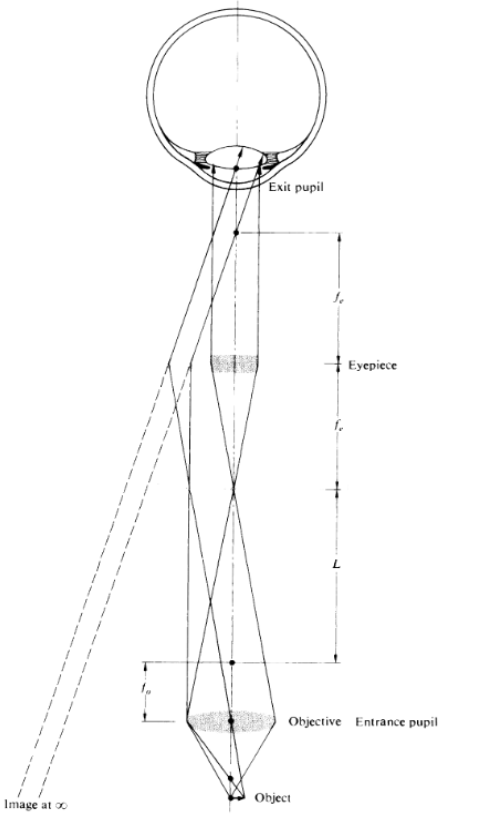
\includegraphics[width=0.4\textwidth]{afbeeldingen/compound_microscope.png}
  	\caption{Schematic drawing of a compound microscope. $f_{e}$ and $f_{o}$ correspond to respectively to the focussing distance of the eyepiece and objective. This figure was apdapted from Hecht, 2016 \cite{hecht}.}
  	\label{fig_compound_microscope}
\end{wrapfigure}

\subsection{Microscopy}
Most modern microscopes are compound microscopes which can achieve a relatively high angular magnification for nearby objects (\cite{hecht}). See figure \ref{fig_compound_microscope} for a schematic drawing of a basic compound microscope.\\
Polarizing microscopes are a type of microscopes that make use of polarizing windows. A polariser is placed in between the light source and the sample and an analyser is placed after the sample. Since the polariser and analyser block all the light except for one specific light polarization, they allow the viewer to see some of the sample's optical properties such as birefringence. \\

\subsection{size measurements}
In this experiment it was chosen to use a CCD camera to record the imaged from the microscope. To measure distances in a sample it is possible to convert a distance in pixels, $n_{pixels}$, to physical units such as meters. For this, we need a conversion factor that gives the length in meters per pixel, $l_{pixel}$. The physical distance, $d_{physical}$ can easily be calculated using equation \ref{eq_distance}.
The value for $l_{pixel}$ should be larger for greater magnifying power.\\

\begin{equation}
	\label{eq_distance}
	d_{physical} = l_{pixel} \cdot n_{pixels}
\end{equation}

\bigskip
\vspace{5mm}

One of the purposes of this experiment is to find out if it is possible to do microscopic measurements with the given microscope. Human hairs and glass fibres have a diameter in the range of 10 - 100 $\mu m$. Measuring the diameter could give insights into the suitability of the given microscope for measurements of this scale.\\
Another purpose for a microscope could be to find sizes of many particles. From this information one could get the average particle size and the distribution for these values. Starch particles have a size up to 100 $\mu m$ and are often ellipse-shaped (\cite{starch}). The size of ellipse-shaped starch particles will be measured in this experiment. The cross section of a particle, $A$, can be calculated using the major and minor diameter of the ellipse, respectively $a$ and $b$, and equation \ref{eq_ellipse}.

\begin{equation}
	\label{eq_ellipse}
	A = 1/4 \cdot a \cdot b \cdot \pi
\end{equation}
\clearpage

\subsection{Birefringence}

Birefringence is an optical property that arises when the refractive index depends on the polarization of incoming light. The quantity birefringence, $\Delta n$, is characterized as the maximum difference between refractive indices (\cite{hecht}). \\

\begin{wrapfigure}{r}{0.5\textwidth}
	\centering
	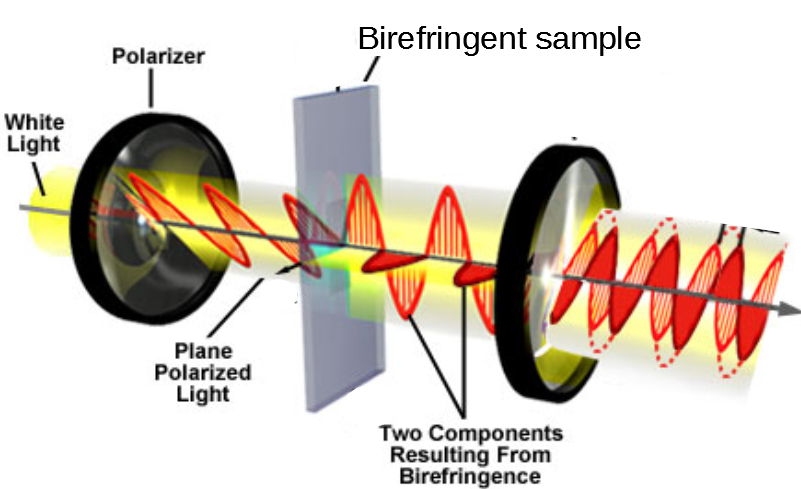
\includegraphics[width=0.45\textwidth]{afbeeldingen/bf_principle.png}
	\caption{Schematic diagram of birefringence between two crossed polarizing windows. This figure was adapted from Olympus, 2012 \cite{olympus}.}
	\label{fig_bf_diagram}
\end{wrapfigure}

When a birefringent material is viewed in a polarizing microscope with the polariser and analyser crossed, bright colours may be observed. The polarized light entering the sample can be decomposed into two orthogonal components, which will experience a different refractive index due to the birefringent properties. The difference in refractive index will result in a path difference, $\Delta l_{path}$, between the two orthogonal components. When these two components interfere, the sum of the two might have changed from polarisation direction, allowing the light to pass the analyser. A schematic diagram of this process can be seen in figure \ref{fig_bf_diagram}. \\
$\Delta l_{path}$ depends on the thickness of the sample, $D$, but also on the wavelength of the light (\cite{hecht}). This means that, for a specific thickness of the sample, the sample will result in positive interference for one wavelength and (partially) negative interference for the others. Subsequently, one colour will be observed for a specific sample thickness.\\
A colour on a Michel-L\'evy colour chart (\cite{bf_chart}) corresponds to a value for $\Delta l_{path}$. Subsequently, the value for $\Delta n$ can be determined using equation \eqref{eq_bf} (\cite{hecht}).

\begin{equation}
	\label{eq_bf}
	\Delta l_{path} = D \cdot \Delta n
\end{equation}


\bigskip
\vspace{5mm}


\subsection{Computerized image improvement}
One of the goals of the experiment is to devise and test digital filters to improve image quality, such as contrast and noise removal.\\
Image features are easier to distinguish if the contrast is high. A way of quantitatively expressing image contrast is through a histogram as outlined in the NI Vision article \cite{histogram_theory}. As illustrated by the two grayscale images in figure \ref{fig:hcphoto} and \ref{fig:lcphoto}, the high contrast image in figure \ref{fig:hcphoto}, has pixel intensity peaks that are more spread over whole intensity range. The contrast of figure \ref{fig:hcphoto} is therefore higher than in figure \ref{fig:lcphoto}. One way to improve contrast is by applying a contrast improving function on the pixel values of an image.\\

\begin{figure}[h!]
    \centering
    \begin{minipage}{.5\textwidth}
      \centering
      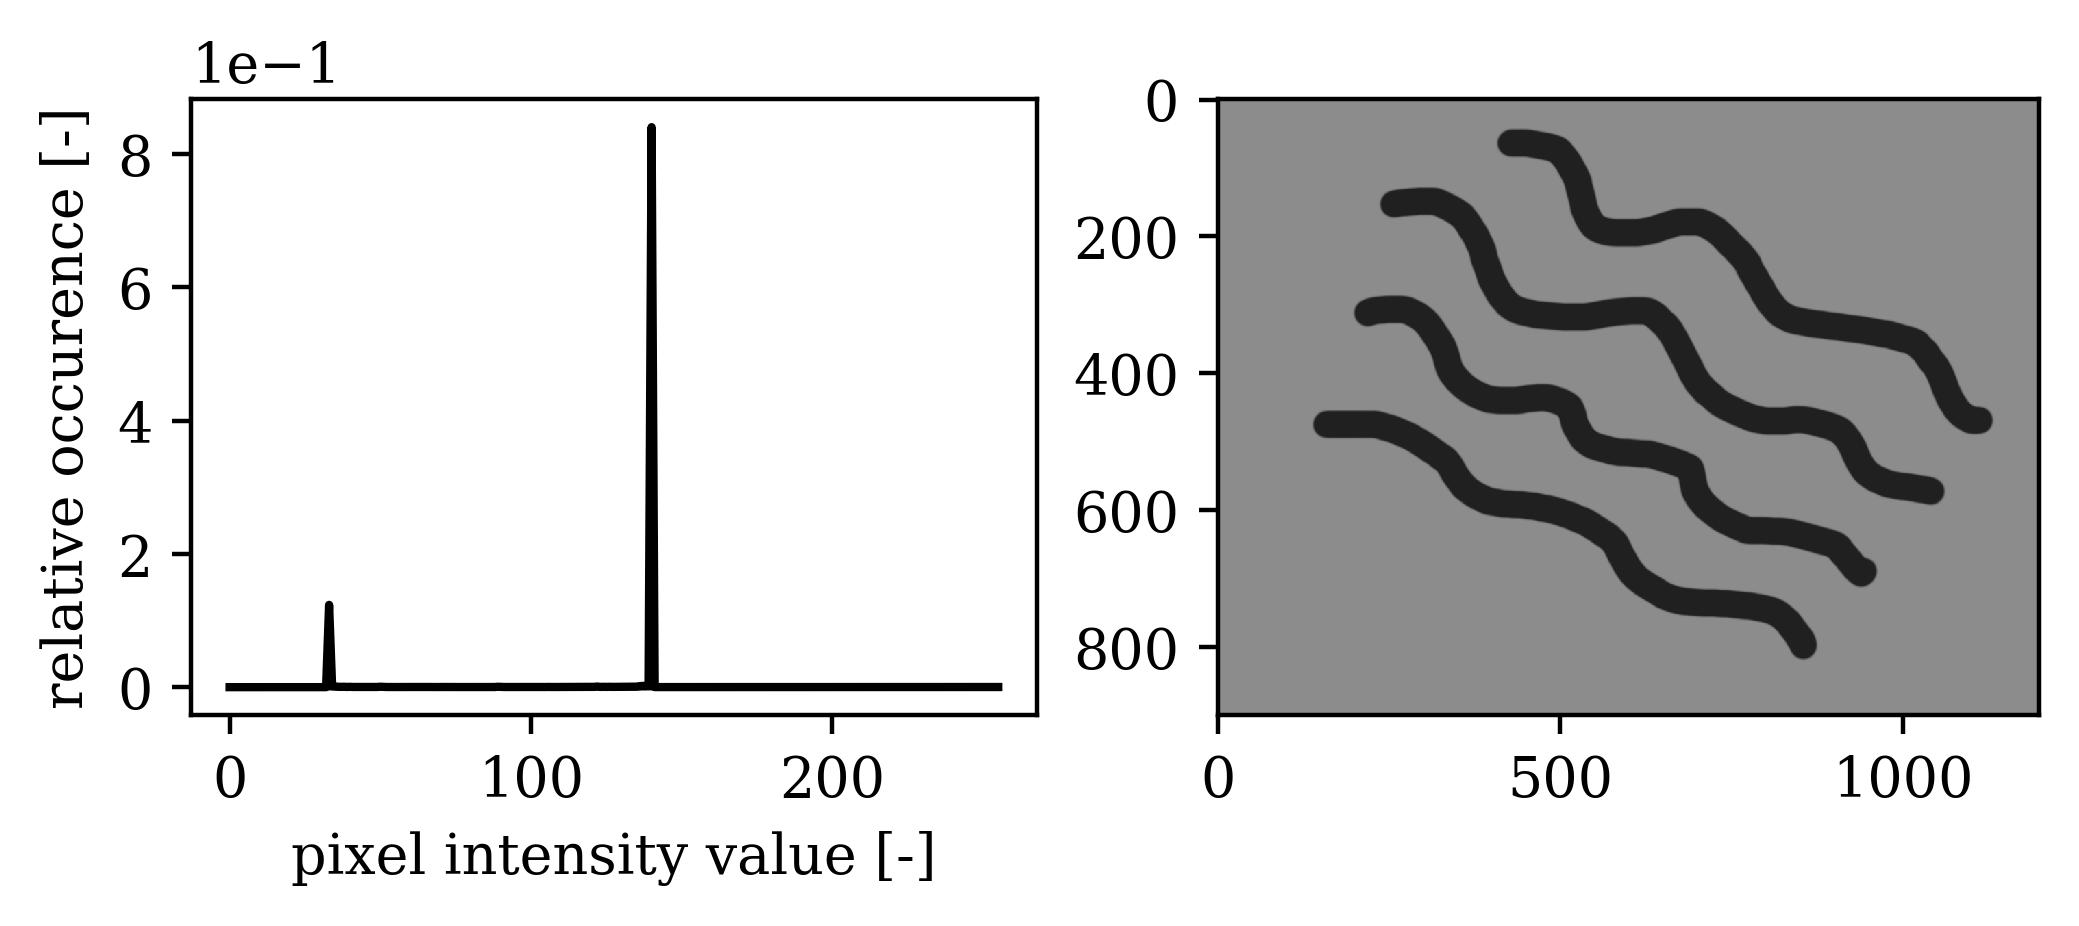
\includegraphics[width=0.9\textwidth,keepaspectratio]{afbeeldingen/histograms/highcontrast.png}
      \caption{High contrast photo}
      \label{fig:hcphoto}
    \end{minipage}%
    \begin{minipage}{.5\textwidth}
      \centering
      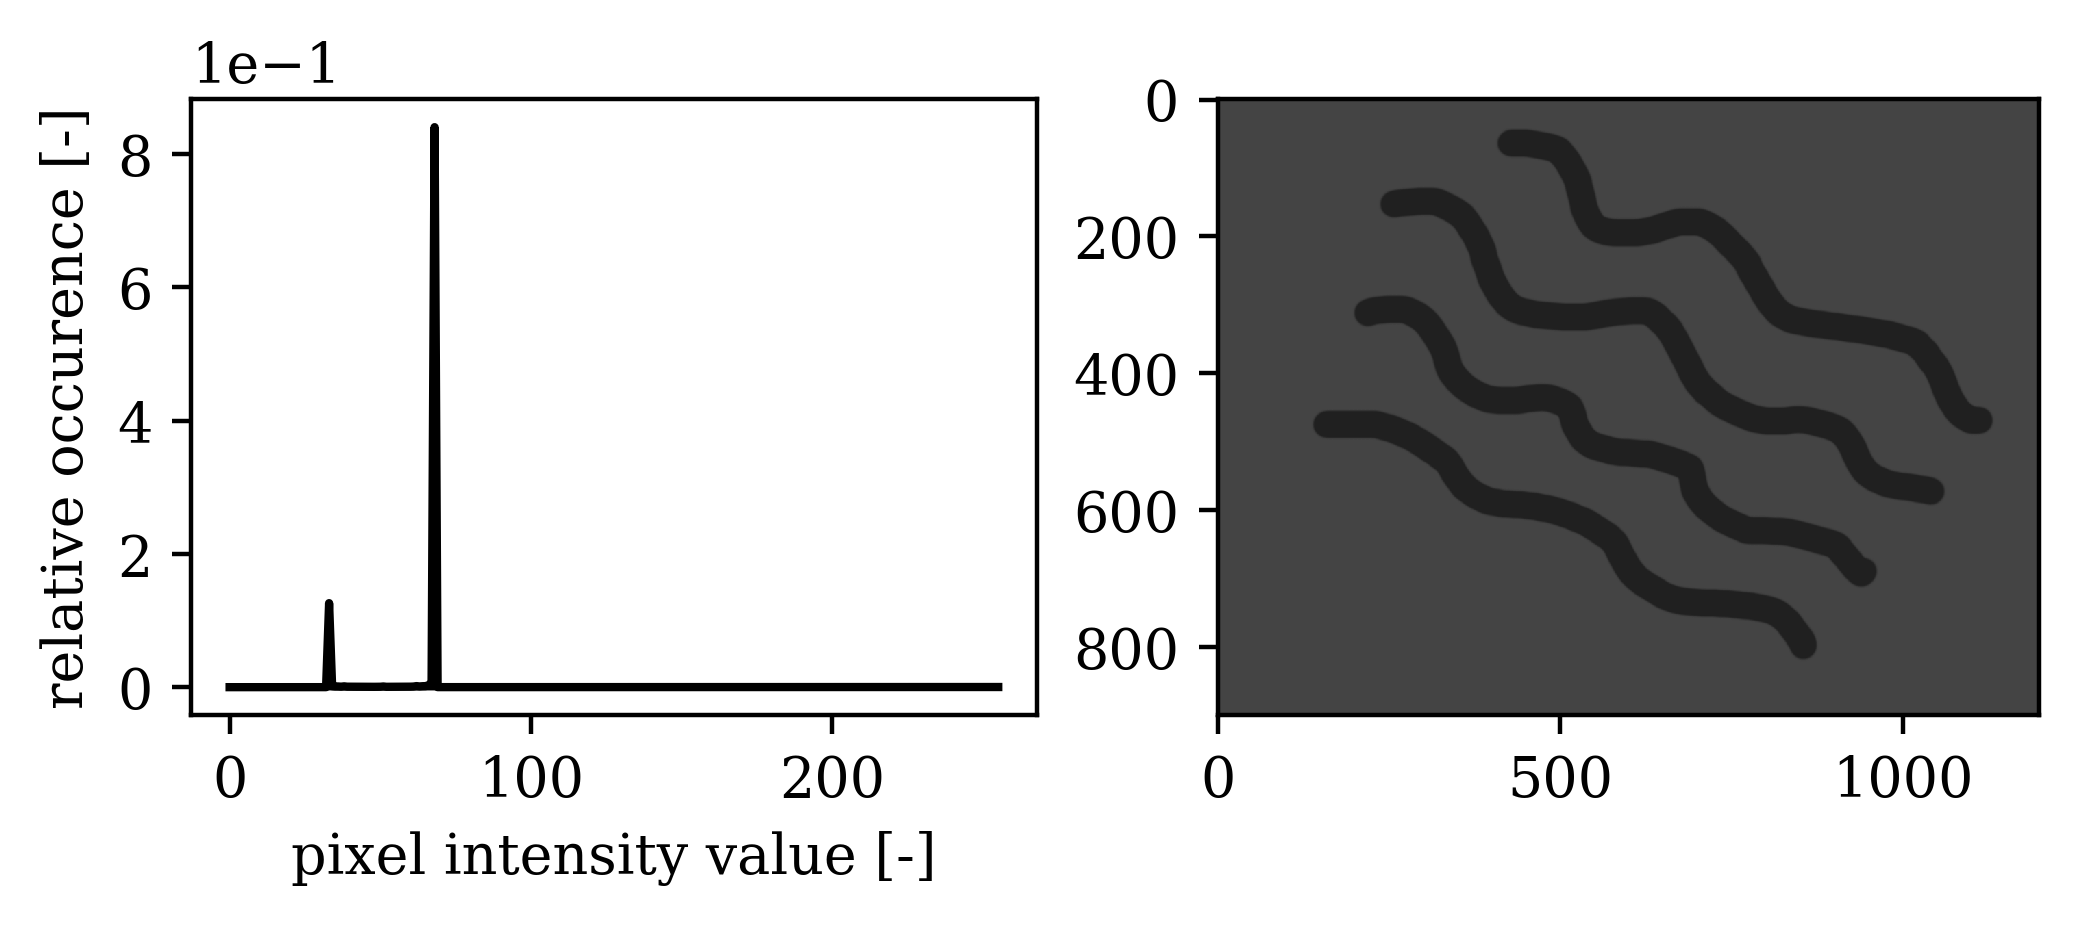
\includegraphics[width=0.9\textwidth,keepaspectratio]{afbeeldingen/histograms/lowcontrast.png}
      \caption{Low contrast photo}
      \label{fig:lcphoto}
    \end{minipage}
\end{figure}

Noise is a phenomenon that cannot be evaded. However, some of the noise can be removed by digital filters, such as rank, median and NxN filters (\cite{tutorial}). \\
Some images suffer from unwanted information, such as uneven illumination or shot noise. Some of this can easily be removed since they only  occur in another frequency-domain than the information we are interested in. One way to select only wanted frequencies is by using Fourier transformations.\\
\\
In this experiment, the sigmoid function to improve contrast and the rank filters from the python skimage package are studied and to what extend they can be used to improve an image.\\



\subsection{Error calculation}

If $Y$ is a variable which is a function of $A$,$B$,$C$, ... Then the error of $Y$, $u(Y)$, is given by equation \ref{eq_error}.

\begin{equation}
	\label{eq_error}
	u(Y) = \sqrt{\left(u(A) \frac{\partial Y}{\partial A}\right)^2 + \left(u(B) \frac{\partial Y}{\partial B}\right)^2 + \left(u(C) \frac{\partial Y}{\partial C}\right)^2 + ...}
\end{equation}

From this it follows that $u(d_{physical})$, $u(A)$ and $u(\Delta n)$, are given respectively by equations \ref{eq_u_distance}, \ref{eq_u_ellipse} and \ref{eq_u_bf}.

\begin{equation}
	\label{eq_u_distance}
	u(d_{physical}) = \sqrt{\left( u(l_{pixel}) \cdot n_{pixels} \right)^2 + \left( u(n_{pixels}) \cdot l_{pixel} \right)^2}
\end{equation}

\begin{equation}
	\label{eq_u_ellipse}
	u(A) = 1/4 \cdot \pi  \sqrt{(u(a) \cdot b)^2 + (u(b) \cdot a)^2}
\end{equation}

\begin{equation}
	\label{eq_u_bf}
	u(\Delta n) = \sqrt{\left( u(\Delta l_{path}) \cdot \frac{1}{D}\right)^2 + \left( u(D) \cdot \frac{l_{path}}{D^2}\right)^2}
\end{equation}
